% !TEX root = ../paper.tex

\begin{itemize}
  \item smooth MMS problem - second-order convergence (based on length, could be a summary at the beginning of the results section + appendix)
  \item 1-D, 2-D void-to-absorber (normally-incident)
  \item 2-D obstruction test problem
  \item 1-D source-in-void test problem
  \item 1-D interface or three-region test problem
\end{itemize}

This section presents results for a number of test problems, which compare
solutions obtained using:
\begin{itemize}
  \item the standard Galerkin FEM, titled in plots as ``Galerkin'',
  \item the low-order method, titled in plots as ``Low'',
  \item the entropy viscosity method, titled in plots as ``EV'',
  \item the standard Galerkin FEM with FCT, titled in plots as ``Galerkin-FCT'', and
  \item the entropy viscosity method with FCT, titled in plots as ``EV-FCT''.
\end{itemize}

%===============================================================================
\subsection{Spatial Convergence}
%===============================================================================

\begin{figure}[htb]
   \centering
      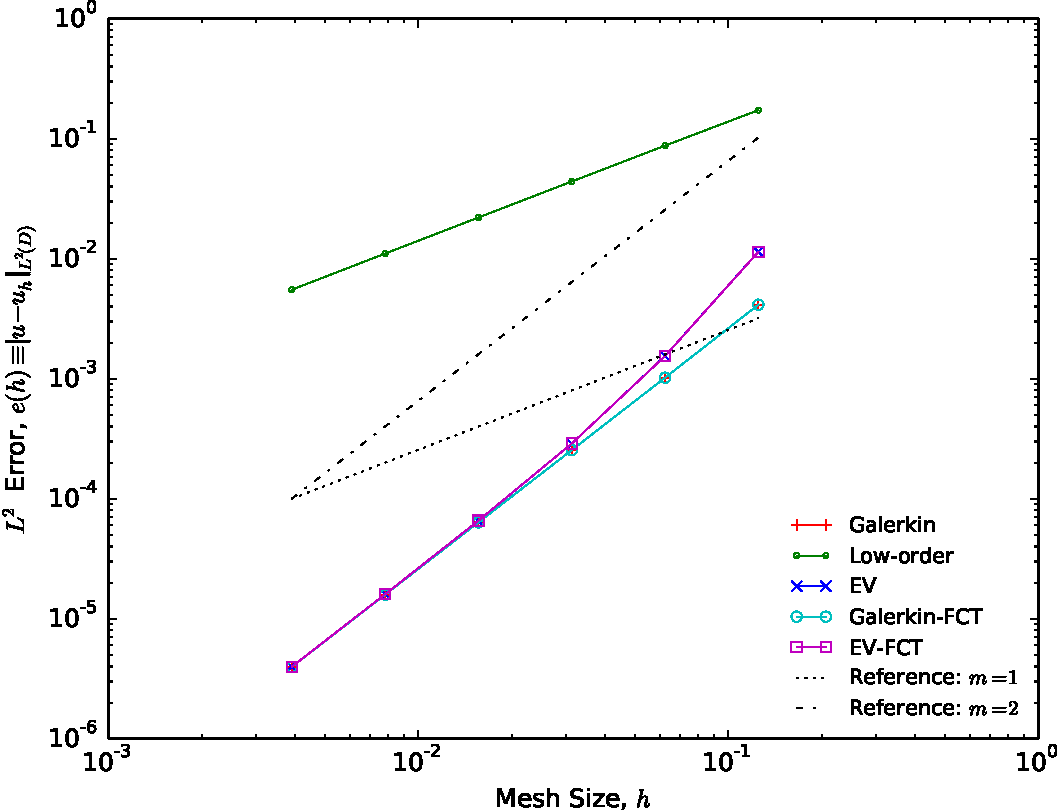
\includegraphics[width=\textwidth]
        {images/convergence_sinx.pdf}
      \caption{Spatial Convergence for MMS Problem}
   \label{fig:mms_sinx_ss}
\end{figure}
\clearpage
%===============================================================================
\subsection{Glancing Beam in a Void}
%===============================================================================
\begin{figure}[ht]
   \centering
   \begin{subfigure}{0.45\textwidth}
      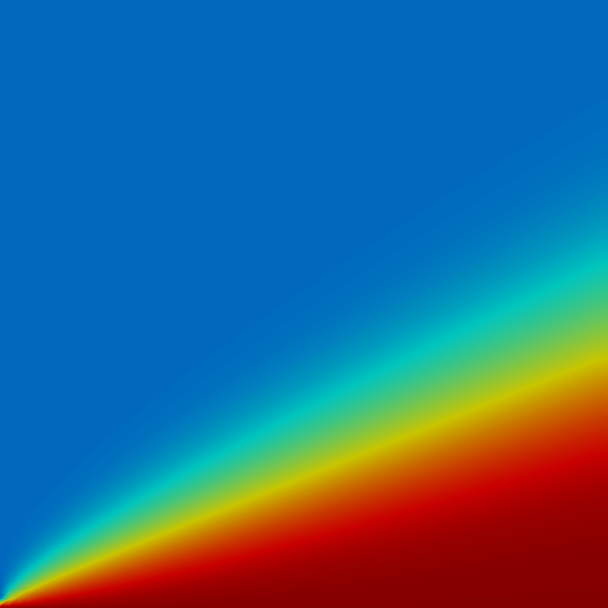
\includegraphics[width=\textwidth]
        {images/glance_Low.png}
      \caption{Low-Order}
   \end{subfigure}
   \begin{subfigure}{0.45\textwidth}
      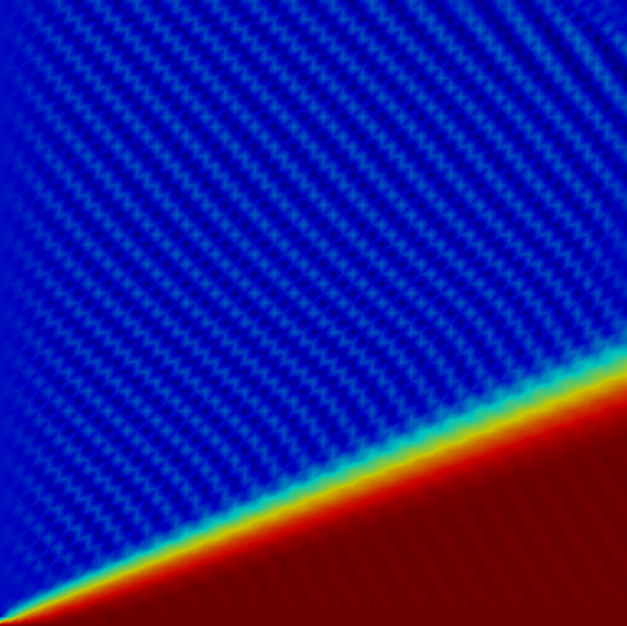
\includegraphics[width=\textwidth]
        {images/glance_EV.png}
      \caption{EV}
   \end{subfigure}
   \begin{subfigure}{0.45\textwidth}
      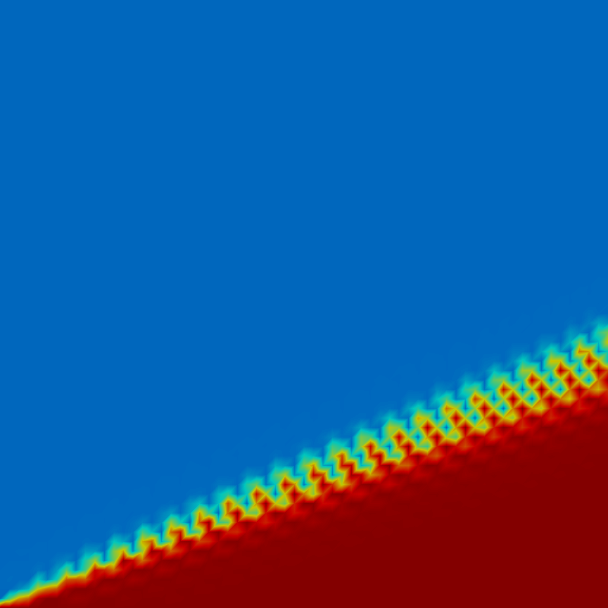
\includegraphics[width=\textwidth]
        {images/glance_GalFCT.png}
      \caption{Galerkin-FCT}
   \end{subfigure}
   \begin{subfigure}{0.45\textwidth}
      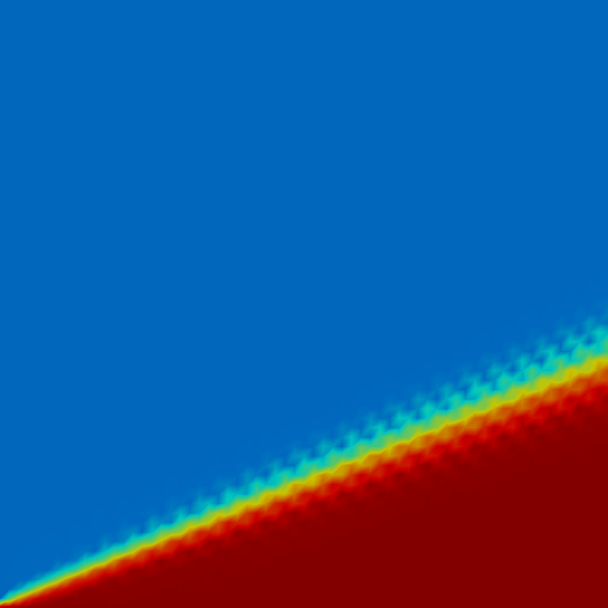
\includegraphics[width=\textwidth]
        {images/glance_EVFCT.png}
      \caption{EV-FCT}
   \end{subfigure}
   \caption{Comparison of Solutions for the Glance-in-Void Test
     Problem Using Explicit Euler Time Discretization}
   \label{fig:glance_in_void_fe}
\end{figure}
\clearpage
%===============================================================================
\subsection{Obstruction}
%===============================================================================
\begin{figure}[ht]
   \centering
   \begin{subfigure}{0.3\textwidth}
      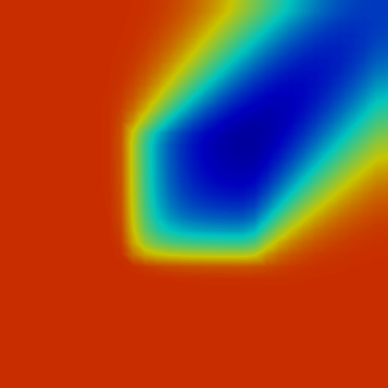
\includegraphics[width=\textwidth]
        {images/obstruction_low.png}
      \caption{Low-Order}
   \end{subfigure}
   \begin{subfigure}{0.3\textwidth}
      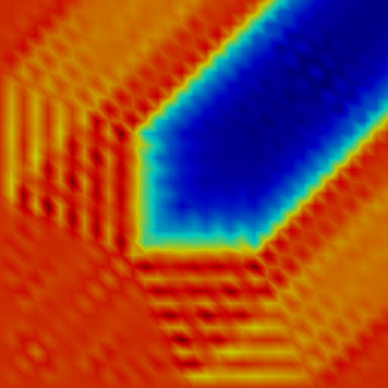
\includegraphics[width=\textwidth]
        {images/obstruction_Gal.png}
      \caption{Galerkin}
   \end{subfigure}
   \begin{subfigure}{0.3\textwidth}
      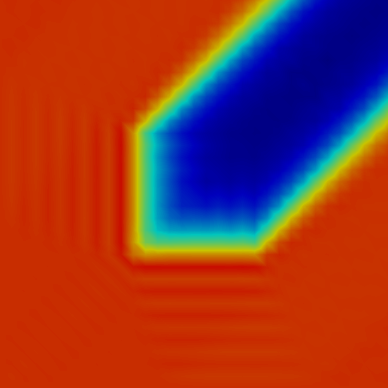
\includegraphics[width=\textwidth]
        {images/obstruction_EV.png}
      \caption{EV}
   \end{subfigure}
   \begin{subfigure}{0.3\textwidth}
      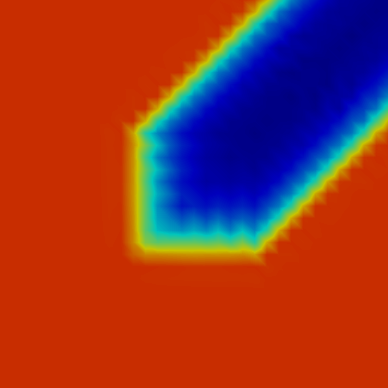
\includegraphics[width=\textwidth]
        {images/obstruction_GalFCT.png}
      \caption{Galerkin-FCT}
   \end{subfigure}
   \begin{subfigure}{0.3\textwidth}
      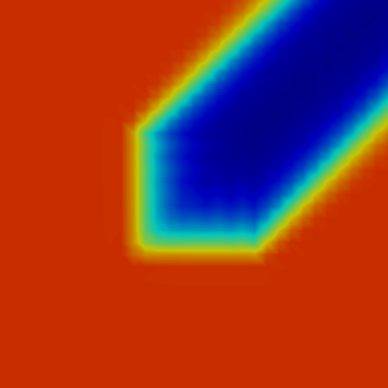
\includegraphics[width=\textwidth]
        {images/obstruction_EVFCT.png}
      \caption{EV-FCT}
   \end{subfigure}
   \caption{Comparison of Solutions for the Obstruction Test
     Problem Using Implicit Euler Time Discretization}
   \label{fig:obstruction_be}
\end{figure}
\clearpage
%===============================================================================
\subsection{Two-Region Interface}
%===============================================================================
\begin{figure}[htb]
   \centering
      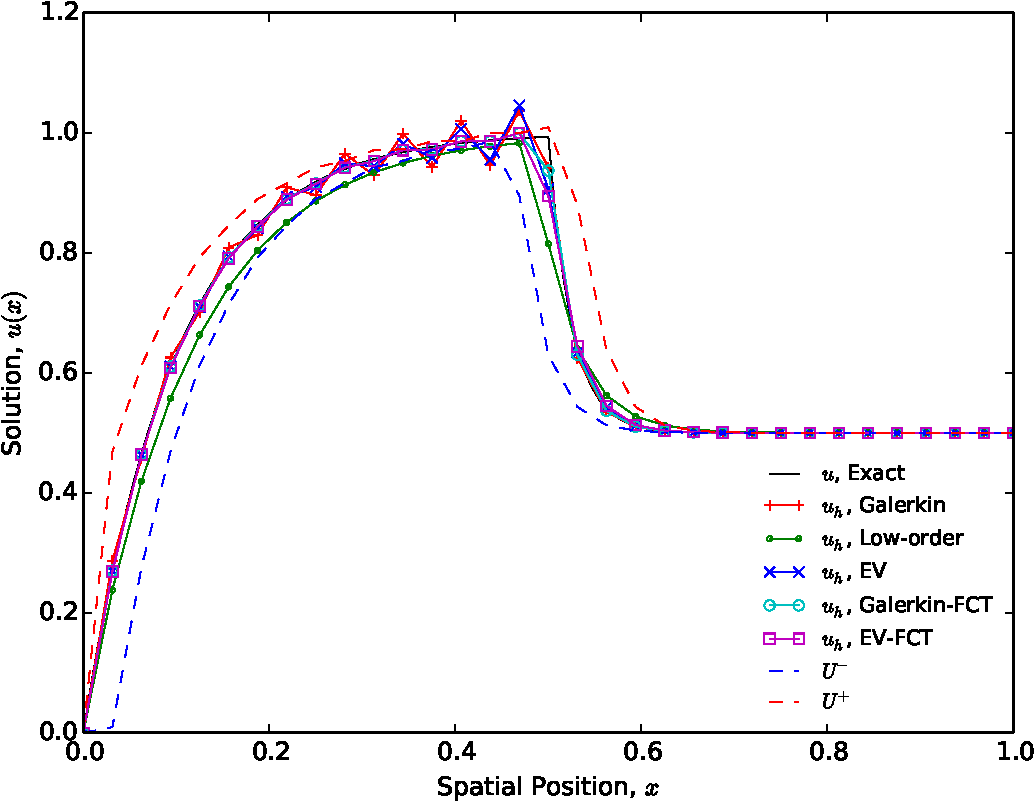
\includegraphics[width=\textwidth]
        {images/solution_interface.pdf}
      \caption{Comparison of Solutions for the Two-Region Interface Test
       Problem Using SSPRK33 Time Discretization}
   \label{fig:interface}
\end{figure}
\clearpage
%===============================================================================
\subsection{Source in a Void}
%===============================================================================
%solution_source_in_void.pdf
\begin{figure}[htb]
   \centering
      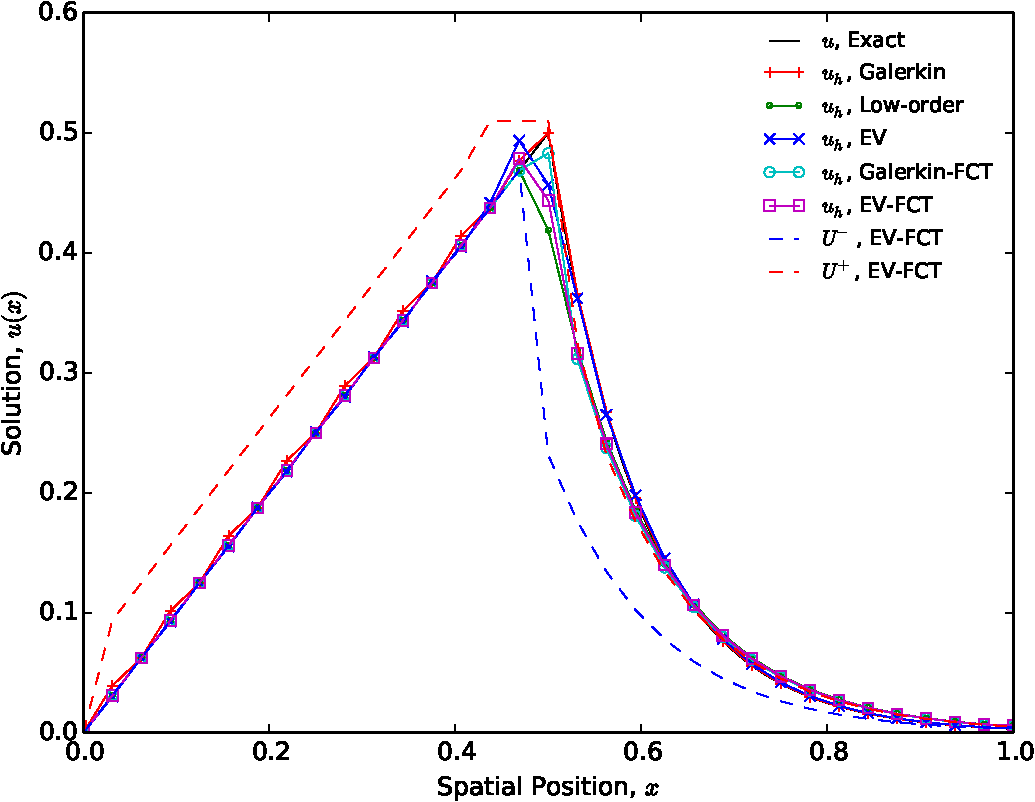
\includegraphics[width=\textwidth]
        {images/solution_source_in_void.pdf}
      \caption{Comparison of Solutions for the Source-in-Void Test
       Problem Using Steady-State Time Discretization}
   \label{fig:source_}
\end{figure}
\clearpage
